\documentclass[8pt]{extarticle}

% Packages
\usepackage[T1]{fontenc}
\usepackage[utf8]{inputenc}
\usepackage{geometry}
\usepackage{multicol} 
\usepackage{xcolor}
\usepackage{listings} %for SQL snippets
\usepackage{pdflscape} % for landscape pages
\usepackage{enumitem} %for formatting of lists
\usepackage{graphicx} %for scaling tabular environments

\usepackage{lipsum} %for sample paragraphs, delete at end


% Page configuration
\geometry{a4paper, landscape, top=10mm, bottom=10mm, left=10mm, right=10mm, columnsep=10mm,}

% no indent globally
\setlength{\parindent}{0pt}

% SQL snippet environment
\lstdefinestyle{sql}{
    language=SQL,
    basicstyle=\small\ttfamily,
    keywordstyle=\color{blue},
    commentstyle=\color{green!40!black},
    stringstyle=\color{red},
    breaklines=true,
    showstringspaces=false,
    tabsize=4,
    numbers=none,
    morekeywords={USE}
}

% Lined separator for headings
\newcommand{\heading}[1]{%
    \noindent
    \rule{\linewidth}{0.4pt}
    \begin{center}
        \vspace{-1ex}
        \textbf{#1}        
        \vspace{-2.5ex}
    \end{center}
    \rule{\linewidth}{0.4pt}
}


\begin{document}

% Remove page numbers for this page
\thispagestyle{empty} 

% Title
\begin{center}   
{\huge\textbf{SQL Cheat Sheet}}\\
\vspace*{0.25cm}
(The running example will be a library database with books. Later on, we introduce a reviews table to perform joins.)\\
\vspace*{0.1cm}
More information can be found in the MySQL docs: https://dev.mysql.com/doc/refman/8.0/en/
\vspace*{0.5cm}
\end{center}

\begin{multicols}{4}
\setlength{\columnseprule}{1pt} % Add vertical line between columns


\heading{SETTING UP DATABASES}

Before creating tables etc. we need somewhere to store them. This is done inside a database. They are created as follows:

\vspace{0.5ex}
\begin{lstlisting}[style=sql]
CREATE DATABASE library;
\end{lstlisting}
\vspace{0.5ex}

To delete a database we use:

\vspace{0.5ex}
\begin{lstlisting}[style=sql]
DELETE DATABASE library;
\end{lstlisting}
\vspace{0.5ex}

Once we create a database we need to enter it before we can create tables etc. We do this via:

\vspace{0.5ex}
\begin{lstlisting}[style=sql]
USE library;
\end{lstlisting}
\vspace{0.5ex}

Note: `USE' and \textcolor{red}{not} `USE DATABASE'.\\

\heading{DATATYPES}

When creating tables, columns are given a datatype. Some common types are:
\begin{itemize}[leftmargin=*]
    \item VARCHAR(n) - variable-length strings with up to $n$ characters.
    \item INT or INTEGER - stores integers.
    \item DECIMAL(n,d) - numbers with $n$ digits, $d$ of which occur after the decimal point.
    \item DATETIME - stores datetimes in the format `YYYY-MM-DD hh:mm:ss'. Functions can be used to extract information (see later).
\end{itemize}

\vspace{1ex}
\heading{SETTING UP TABLES}

To create a table, we pass a name for the table and a list of column names along with their datatypes. Let's create a `books' table for our library database.

\vspace{0.5ex}
\begin{lstlisting}[style=sql]
CREATE TABLE books (
    title VARCHAR(30),
    author VARCHAR(30),
    pages INT
);
\end{lstlisting}
\vspace{0.5ex}

We can drop (or delete) unwanted tables using:

\vspace{0.5ex}
\begin{lstlisting}[style=sql]
DROP TABLE books;
\end{lstlisting}
\vspace{0.5ex}

We may describe tables using 

\vspace{0.5ex}
\begin{lstlisting}[style=sql]
DESC books;
\end{lstlisting}
\vspace{0.5ex}

 This query gives the following output:
 
 \vspace{1.5ex}
 \resizebox{\columnwidth}{!}{%
   \begin{tabular}{|c|c|c|c|c|c|}
   \hline
        Field & Type & Null & Key & Default & Extra  \\
        \hline
        title & varchar(30) & YES &&NULL& \\
        author & varchar(30) & YES &&NULL&\\
        pages & int & YES &&NULL&\\
        \hline
    \end{tabular} %
}
\vspace*{1.5ex}

\heading{NULL, KEY, DEFAULT \& EXTRA?}

The other four columns in the desc table give the following information:
\begin{itemize}[leftmargin=*]
    \item NULL: use `NOT NULL' after datatype in table creation to ensure values inserted into the table cannot be null
    \item Key: If the column is a primary key (use PRIMARY KEY in initialisation), or has a uniqueness constraint on it (UNIQUE) etc
    \item Default: If no value is specified, what should the column value be set to by default (DEFAULT $\ldots$ in initialisation)
    \item Extra: extra information, such as whether the column has auto-increment is included here (e.g. AUTO$\_$INCREMENT in the initialisation.)
\end{itemize}

\vspace*{1.5ex}

\heading{CONSTRAINTS ON COLUMNS}

Some constraints that can be put on columns are:
\begin{itemize}[leftmargin=*]
    \item NOT NULL - values in this column cannot be null.
    \item UNIQUE - values in this column must be unique.
    \item PRIMARY KEY - NOT NULL + UNIQUE, this uniquely identifies a row. (For books this could be the ISBN, for example.)
    \item DEFAULT - sets a default value if no value is passed.
    \item CHECK - ensures values satisfy a certain condition.
\end{itemize}

Let's drop and recreate our `books' table with some reasonable constraints.

\vspace{0.5ex}
\begin{lstlisting}[style=sql]
DROP TABLE books;

CREATE TABLE books (
id INT PRIMARY KEY AUTO_INCREMENT,
title VARCHAR(30) NOT NULL,
author VARCHAR(30) NOT NULL,
pages INT CHECK (pages > 0) 
);
\end{lstlisting}

\vspace{1ex}

\heading{INSERTING INTO TABLES}

We insert rows into tables using `VALUES'. Columns with the NOT NULL constraint must be given a value, columns which auto increment do not need a value passed as this is handled automatically. 

\vspace{0.5ex}
\begin{lstlisting}[style=sql]
INSERT INTO books 
    (title, author, pages)
VALUES 
    ('Great Expectations', 'Charles Dickens', 544),
    ('1984', 'George Orwell', 311);
\end{lstlisting}
\vspace{0.5ex}

\vspace{1ex}

\heading{SELECT}

We may view our table using SELECT. The query SELECT * allows us to view all columns.

\vspace{0.5ex}
\begin{lstlisting}[style=sql]
SELECT * FROM books;
\end{lstlisting}
\vspace{0.5ex}

Output:

\vspace{1.5ex}
 \resizebox{\columnwidth}{!}{%
   \begin{tabular}{|c|c|c|c|c|c|}
   \hline
        id & title & author & pages  \\
        \hline
        1 & Great Expectations & Charles Dickens & 544 \\
        2 & 1984 & George Orwell & 311\\
        \hline
    \end{tabular} %
}
\vspace*{1.5ex}

SELECT [column names] allows us to view some of the columns. We may also relabel columns (temporarily, as part of the output only) using AS. For example: 

\vspace{0.5ex}
\begin{lstlisting}[style=sql]
SELECT title AS book_title FROM books;
\end{lstlisting}
\vspace{0.5ex}

Output:
\begin{center}
\resizebox{0.45\columnwidth}{!}{%
   \begin{tabular}{|c|c|}
   \hline
        book\_title \\
        \hline
        Great Expectations\\
        George Orwell\\
        \hline
    \end{tabular} %
}    
\end{center} 
\vspace*{1.5ex}

Furthermore, we may use the WHERE clause to only return rows which satisfy current conditions. For example, the query

\vspace{0.5ex}
\begin{lstlisting}[style=sql]
SELECT * FROM books WHERE id = 1;
\end{lstlisting}
\vspace{0.5ex}

gives the output:


\vspace{1.5ex}
 \resizebox{\columnwidth}{!}{%
   \begin{tabular}{|c|c|c|c|c|c|}
   \hline
        id & title & author & pages  \\
        \hline
        1 & Great Expectations & Charles Dickens & 544 \\
        \hline
    \end{tabular} %
}
\vspace*{1.5ex}

Some comparisons we may use with the WHERE clause include <, >, =, !=, BETWEEN, OR, AND, LIKE, IN, IS NULL $\ldots$. For the most part the word NOT can go in front of these words.\\

Subqueries also work well with the WHERE clause. The inner query is completed first, to be used within the main query. As a silly example, this query gives the same output as above:

\vspace{0.5ex}
\begin{lstlisting}[style=sql]
SELECT *
FROM books
WHERE id =
    (
        SELECT id FROM books WHERE title LIKE 'G%'
    );
\end{lstlisting}
\vspace{0.5ex}

\vspace{1ex}

\heading{UPDATING ROWS WITHIN TABLES}

We update rows in tables using queries of the form 

\vspace{0.5ex}
\begin{lstlisting}[style=sql]
UPDATE table_name
SET column_name = something 
WHERE condition;
\end{lstlisting}
\vspace{0.5ex}

Primary keys work well with the WHERE clause when wanting to update a specific row. For example, if we later discovered that `1984' has $312$ pages and not $311$ we may update this row using its unique identifier `id = 2' as follows

\vspace{0.5ex}
\begin{lstlisting}[style=sql]
UPDATE books 
SET pages = 312 
WHERE id = 2;
\end{lstlisting}
\vspace{0.5ex}

\vspace{1ex}

\end{multicols}

\newpage
% Remove page numbers for this page
\thispagestyle{empty} 

\begin{multicols}{4}
\setlength{\columnseprule}{1pt} % Add vertical line between columns
\heading{DELETING ROWS WITHIN TABLES}

We delete rows in tables using queries of the form 

\vspace{0.5ex}
\begin{lstlisting}[style=sql]
DELETE FROM table_name 
WHERE condition;
\end{lstlisting}
\vspace{0.5ex}

For example, if we only wanted to stock books with less than $500$ pages in our library, and wanted to update our table accordingly, we could perform the query.

\vspace{0.5ex}
\begin{lstlisting}[style=sql]
DELETE FROM books
WHERE pages >= 500;
\end{lstlisting}
\vspace{0.5ex}


\heading{ALTERING TABLES}

We may alter tables using the ALTER TABLE keyword. Examples of things we can do are:

\begin{itemize}
    \item ADD \ldots; (adds a column)
    \item ADD COLUMN \ldots; (same as above)
    \item DROP COLUMN \ldots;
    \item RENAME COLUMN \ldots TO \ldots;
    \item MODIFY COLUMN \ldots; (to change datatype of existing column, for example)
\end{itemize}

\vspace{1ex} 
\heading{FUNCTIONS ON DATATYPES}

We may perform functions on datatypes (as part of the output). Functions on strings include:
\begin{itemize}[leftmargin=*]
    \item CONCAT: concatenates strings together.
    \item SUBSTRING or SUBSTR: extract substring from a string.
    \item UPPER: replaces all characters with their upper case counterpart.
    \item LOWER: replaces all characters with their lowercase counterpart.
    \item CHAR\_LENGTH: returns the number of characters in the string as an integer. Note that this is not the same as the LENGTH function, which may produce unexpected results when considering multi-byte characters.
\end{itemize}

For example, the following query creates a sentence from each row in the table, making use of the CONCAT string function. 

\vspace{0.5ex}
\begin{lstlisting}[style=sql]
SELECT 
    CONCAT(title, ' was written by ', author) AS title_and_author
FROM
    books;
\end{lstlisting}
\vspace{1ex}

Output:

\vspace{2ex}
 \resizebox{\columnwidth}{!}{%
   \begin{tabular}{|c|}
   \hline
   title\_and\_author \\
   \hline
    Great Expectations was written by Charles Dickens \\
    \hline
    1984 was written by George Orwell \\
    \hline
    \end{tabular} %
    }
\vspace*{2ex}

There exist functions for other datatypes, for example, the datetime datatype has functions such as DAYNAME, MONTH, YEAR, HOUR, $\ldots$. See documentation for more.
\vspace{1ex}

\heading{REFINING SELECT QUERIES}

We may refine SELECT queries using keywords such as DISTINCT, ORDER BY, and LIMIT. We see some examples. First, we add another row to the table, obtaining the following. 

\vspace{1.5ex}
 \resizebox{\columnwidth}{!}{%
   \begin{tabular}{|c|c|c|c|}
   \hline
   id & title & author & pages \\
   \hline
    1 & Great Expectations & Charles Dickens & $544$\\
    \hline
    2 & 1984 & George Orwell & $311$\\
    \hline
    3 & Oliver Twist & Charles Dickens & $608$\\
    \hline
    \end{tabular} %
    }
\vspace*{0.5ex}

\vspace{0.5ex}
\begin{lstlisting}[style=sql]
SELECT DISTINCT author
FROM books;
\end{lstlisting}
\vspace{0.5ex}

Output:
\begin{center}
 \resizebox{0.35\columnwidth}{!}{%
   \begin{tabular}{|c|}
   \hline
   author \\
   \hline
    Charles Dickens \\
    \hline
    George Orwell \\
    \hline
    \end{tabular} %
    }    
\end{center}
\vspace*{0.5ex}

\vspace{0.5ex}
\begin{lstlisting}[style=sql]
SELECT title, pages
FROM books
ORDER BY pages DESC;
\end{lstlisting}
\vspace{0.5ex}

This query selects the title and pages of each row, and orders the rows using the number of pages, in descending order.
\vspace{1ex}

Output:
\begin{center}
 \resizebox{0.55\columnwidth}{!}{%
   \begin{tabular}{|c|c|}
   \hline
   title & pages \\
   \hline
   Oliver Twist & 608 \\
   \hline
    Great Expectations & 544\\
    \hline
    1984 & 311 \\
    \hline
    \end{tabular} %
    }    
\end{center}
\vspace*{1.5ex}

\vspace{1ex}

\heading{GROUP BY AND AGGR. FUNCS}

We may group the data within the table using the entries in specific columns. Such a grouping does not preserve the table structure, however, we can perform aggregate functions such as COUNT, AVG, MIN, MAX, and SUM on each group to extract information. 

For example, grouping by `author' gives us the following grouping.
\begin{center}
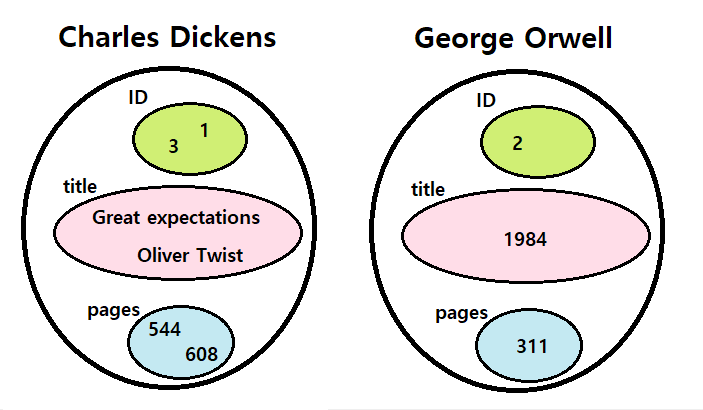
\includegraphics[scale = 0.3]{sql_group_by_visual.png}
\end{center}

Now SELECT queries can make use of `author' and aggregate functions on `id', `title', and `pages'. We cannot query, for example, pages directly since pages are now within groups, and have lost their structure as part of a row.

\vspace{0.5ex}
\begin{lstlisting}[style=sql]
SELECT author, COUNT(title)
FROM books
GROUP BY author;
\end{lstlisting}
\vspace{0.5ex}

This query groups all books in the `books' table using the `author' column, then selects the author along with COUNT(title), i.e. the number of titles in the `title' bubble (see diagram).
\vspace{1ex}

Output:
\begin{center}
 \resizebox{0.8\columnwidth}{!}{%
   \begin{tabular}{|c|c|}
   \hline
   author & COUNT(title) \\
   \hline
   Charles Dickens & 2 \\
   \hline
   George Orwell & 1 \\
   \hline
    \end{tabular} %
    }    
\end{center}
\vspace*{1.5ex}

We can restrict which groups we wish to consider using the HAVING clause. This ensures we select only the groups which satisfy certain properties. For example the query

\vspace{0.5ex}
\begin{lstlisting}[style=sql]
SELECT author, AVG(pages)
FROM books
GROUP BY author
HAVING count(title) >= 2;
\end{lstlisting}
\vspace{0.5ex}

will output a table with the author and the average page count, but only for authors with at least $2$ books. \\

Lastly, we can GROUP BY ... WITH ROLLUP. This does what it says on the tin, it queries within groups based on the given grouping, then `rolls up' or `steps back a level of grouping' and queries again until all levels have been exhausted. For example,

\vspace{0.5ex}
\begin{lstlisting}[style=sql]
SELECT author, count(title).
FROM books
GROUP BY author
WITH ROLLUP;
\end{lstlisting}

gives the output: 
\begin{center}
 \resizebox{0.8\columnwidth}{!}{%
   \begin{tabular}{|c|c|}
   \hline
   author & COUNT(title) \\
   \hline
   Charles Dickens & 2 \\
   \hline
   George Orwell & 1 \\
   \hline
   NULL & 3 \\
   \hline
    \end{tabular} %
    }    
\end{center}
\vspace*{0.25ex}

What has happened is `author' and count have been carried out using the author grouping, and then we have `rolled up', resulting in the trivial grouping (in the diagram, imagine both big bubbles and the corresponding small coloured bubbles merging together) where the query is carried out once again.

\vspace{1ex} 
\heading{VIEWS \& CTEs (VIRTUAL TABLES)}

Views and CTEs (Common Table Expressions) are both `virtual tables' in some sense. The difference is that views are stored in the database (just like regular tables). CTEs are created and exist only within the scope of the query, so they exist only temporarily.

Suppose the | author | COUNT(title) | table (from the GROUP BY section) is something we wish to work with.\\

If we want to work with it frequently we may store it as a view. 


\vspace{0.5ex}
\begin{lstlisting}[style=sql]
CREATE VIEW author_book_count AS (
    SELECT author, COUNT(title)
    FROM books
    GROUP BY author );
\end{lstlisting}
\vspace{0.5ex}

A view is as it says, it is a stored `viewpoint' of the data. Therefore we may read from the view (using SELECT) but we cannot UPDATE or DELETE rows from a view (as this would affect the data in the original table(s)).We can read from it just like we would from a normal table. 

\vspace{0.5ex}
\begin{lstlisting}[style=sql]
SELECT * FROM author_book_count;
\end{lstlisting}
\vspace{0.5ex}

This will produce the same output as the first query within the GROUP BY section. (This should be no surprise since this was the query used to create the view.)

If we want to produce this table and work with it further there-and-then, then creating a CTE may be best.

\vspace{0.5ex}
\begin{lstlisting}[style=sql]
WITH author_book_counts AS (
    SELECT author, COUNT(title) AS book_count
    FROM books
    GROUP BY author
    )
*query involving author_book_counts*;
\end{lstlisting}
\vspace{0.5ex}

\end{multicols}

\newpage
% Remove page numbers for this page
\thispagestyle{empty} 

\begin{multicols}{4}
\setlength{\columnseprule}{1pt} % Add vertical line between columns

\heading{FOREIGN KEYS}

For use in upcoming sections, we produce another table called `reviews'. Each review corresponds to a book, and to signify this in SQL we include a column in `reviews' called `book\_id' (or something meaningful) which references the id of the book in the `books' table. This is done using a foreign key.

\begin{center}
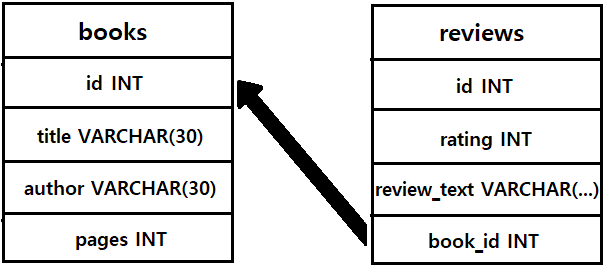
\includegraphics[scale = 0.38]{sql_pointer.png}
\end{center}

\begin{lstlisting}[style=sql]

CREATE TABLE reviews (
    id INT PRIMARY KEY AUTO_INCREMENT,
    rating INT CHECK (rating BETWEEN 0 AND 5),
    review_text VARCHAR(1000) DEFAULT 'No review text',
    book_id INT,
    FOREIGN KEY (book_id) 
        REFERENCES books(id)
);
\end{lstlisting}
\vspace{0.5ex}

We insert two reviews for Oliver Twist (book.id = $3$) into the `reviews' table, producing the following output via a SELECT * query.

\begin{center}
 \resizebox{\columnwidth}{!}{%
   \begin{tabular}{|c|c|c|c|}
   \hline
   id & rating & review\_text & book\_id \\
   \hline
  1 & 4 & Great book & 3 \\
   \hline
   2 & 5 & Couldn't put it down & 3 \\
   \hline
    \end{tabular} %
    }    
\end{center}

\vspace{1ex}
\heading{INNER JOINS \& LEFT/RIGHT JOINS}

The idea behind a join is that we can glue two tables together along a specified column. \\

Inner joins work a bit like the intersection of two sets, $A \cap B$, where only rows with at least one matching row from the other table (along the specified column) will be included. \\

Left joins, in contrast, are like taking the whole set $A$. All rows of the `left table' are taken, and rows of the `right' table are joined onto the `left table' where they match (along the specified column). Right join is analogous, with the roles of left and right reversed.\\

Let's join the `books' table and the `reviews' table along the columns corresponding to the book id. For the `books' table this is column `id' and for the `reviews' table this is column `book\_id'.

\vspace{0.5ex}
\begin{lstlisting}[style=sql]
SELECT *
FROM books
    JOIN reviews
        ON books.id = reviews.book_id;
\end{lstlisting}
\vspace{0.5ex}

This results in the following table (a zoom-in may be required...)
\begin{center}
    \vspace{-1ex}
 \resizebox{\columnwidth}{!}{%
   \begin{tabular}{|c|c|c|c|c|c|c|c|}
   \hline
   id & title & author & pages & id & rating & review\_text & book\_id \\
   \hline
   3 & Oliver Twist & Charles Dickens & 608 & 1 & 4 & Great book & 3 \\
   \hline
   3 & Oliver Twist & Charles Dickens & 608 & 2 & 5 & Couldn't put it down! & 3 \\
   \hline
    \end{tabular} %
    }    
\end{center}

Observe that only `Oliver Twist' appears, as it is the only book with a review. We now do the same thing, but use left join instead of a (inner) join. Notice that all three books appear, with two of them having NULL reviews.

\vspace{0.5ex}
\begin{lstlisting}[style=sql]
SELECT *
FROM books
    LEFT JOIN reviews
        ON books.id = reviews.book_id;
\end{lstlisting}
\vspace{0.5ex}

Output:

\begin{center}
 \resizebox{\columnwidth}{!}{%
   \begin{tabular}{|c|c|c|c|c|c|c|c|}
   \hline
   id & title & author & pages & id & rating & review\_text & book\_id \\
   \hline
    1 & Great Expectations & Charles Dickens & 544 & NULL & NULL & NULL & NULL \\
    \hline
    2 & 1984 & George Orwell & 311 & NULL & NULL & NULL & NULL \\
    \hline   
   3 & Oliver Twist & Charles Dickens & 608 & 1 & 4 & Great book & 3 \\
   \hline
   3 & Oliver Twist & Charles Dickens & 608 & 2 & 5 & Couldn't put it down! & 3 \\
   \hline
    \end{tabular} %
    }    
\end{center}

\vspace{1ex}
\heading{MANY TO MANY JOINS}

For the previous joins, each review belonged to exactly one book. However, some pairs of tables have a many-to-many relationship (e.g. books and reviewers, as a book can have many reviewers, and a reviewer can review many books). \\

In this case, we should use a third table (perhaps called `books\_reviewers') with two columns, named `book\_id' and `reviewer\_id', which are both foreign keys. \\

This third table, along with a double join, can be used to join data from the `books' and `reviewers' tables. \\
For example:

\vspace{0.5ex}
\begin{lstlisting}[style=sql]
SELECT * FROM books
    JOIN books_reviewers
        ON books.id = books_reviewers.book_id
    JOIN reviewers
        ON reviewers.id = books_reviewers.reviewer_id;
\end{lstlisting}
\vspace{0.5ex}

\vspace{1ex}
\heading{WINDOW FUNCTIONS}

Window functions are a little bit like functions on groups, in the sense that we can do calculations on groups of data (however in the case of window functions, these groups are called partitions). \\

The main difference is that the partitions created when performing window functions do not collapse the rows with respect to the grouping (or partition), but instead keep all rows separate and intact.\\

So, when a partition column is specified, all rows are partitioned with respect to this column, with the row structure being preserved. We can perform aggregate functions on the partitions, but also functions which require the rows to be intact, for example, ranking the rows based on an ordering within the partitions.\\

A rough visualisation of this is the following (assuming a partition over the `author' column)

\begin{center}
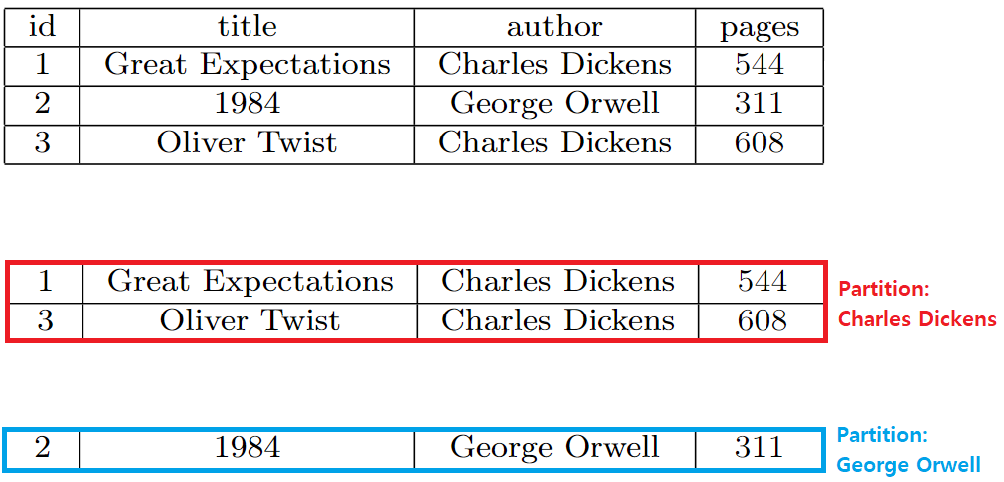
\includegraphics[scale = 0.24]{window_functions.png}
\end{center}

So, window functions can take an aggregate function (e.g. AVG) and produce honest columns in our table, where the value on each row corresponds to the value of the aggregate function on the associated partitioned piece. \\

 Additionally, we can put an order on the partition. This allows us to do things like rank rows within partitions, or label rows by quartiles, or more generally n-tiles, within each partition.

The following query will rank the books by each author from longest to shortest.

\vspace{0.5ex}
\begin{lstlisting}[style=sql]
SELECT *,
       rank() over (partition by author order by pages desc) as author_book_length_rank
FROM books;
\end{lstlisting}
\vspace{0.5ex}

Output:

\begin{center}
 \resizebox{\columnwidth}{!}{%
   \begin{tabular}{|c|c|c|c|c|}
   \hline
   id & title & author & pages & author\_book\_length\_rank \\
   \hline   
   3 & Oliver Twist & Charles Dickens & 608 & 1\\
   \hline
    1 & Great Expectations & Charles Dickens & 544 & 2\\
    \hline
    2 & 1984 & George Orwell & 311 & 1 \\
    \hline
    \end{tabular} %
    }    
\end{center}

How has this happened?\\
The `over (partition by author $\ldots$)' has partitioned the rows by author. Then inside each partition, the rows are ordered with respect to the number of pages, `($\ldots$ order by pages desc)'. The window function `rank()' then returns a rank based on this ordering.\\

Note that the partition belongs to the column, we can make use of different partitions and orderings for different columns.\\

Another example is finding the average book length of the long books (say books with length $> 500$) and the short books. We do this using CASE (not seen elsewhere in the cheat sheet).

\vspace{0.5ex}
\begin{lstlisting}[style=sql]
SELECT title, AVG(pages) OVER (PARTITION BY 
              CASE
                  WHEN pages > 500 THEN 'Long Book'
                  ELSE 'Short Book'
              END) as avg_pages_long_short from books;
\end{lstlisting}

Output:
\vspace{-1.5ex}
\begin{center}
    \resizebox{\columnwidth}{!}{%
    \begin{tabular}{|c|c|c|c|c|}
        \hline
        title & avg\_pages\_long\_short \\
        \hline   
        Great Expectations & 576.0000\\
        \hline
        Oliver Twist &  576.0000\\
        \hline
        1984 & 311.0000 \\
        \hline
    \end{tabular} %
    }    
\end{center}

This works by first partitioning the rows based on whether they are a `long book' or a `short book'. Within these partitions, the average page count is computed and appended to its corresponding row.\\

A list of some window functions are:

\begin{itemize}[leftmargin=*]
    \item Most aggregate functions, such as AVG, COUNT, MIN, MAX. \\If an order by is provided, these functions become rolling functions e.g. SUM becomes a cumulative sum.
    \item rank(): determines the rank with respect to some order (note: order by must be provided).
    \item lead() and lag() (note: order by must be provided).
    \item ntile(n) (note: order by must be provided).
    \item first\_value(), last\_value() (note: order by must be provided).
\end{itemize}

\end{multicols}
\end{document}
